% !TeX TXS-program:bibliography = txs:///biber
\documentclass[14pt, russian]{scrartcl}
\let\counterwithout\relax
\let\counterwithin\relax
%\usepackage{lmodern}
\usepackage{float}
\usepackage{xcolor}
\usepackage{extsizes}
\usepackage{subfig}
\usepackage[export]{adjustbox}
\usepackage{tocvsec2} % возможность менять учитываемую глубину разделов в оглавлении
\usepackage[subfigure]{tocloft}
\usepackage[newfloat]{minted}
\removefromtoclist[float]{lol}% must be after loading `minted`.
\captionsetup[listing]{position=top}

\AtBeginEnvironment{figure}{\vspace{0.5cm}}
\AtBeginEnvironment{table}{\vspace{0.5cm}}
\AtBeginEnvironment{listing}{\vspace{0.5cm}}
\AtBeginEnvironment{algorithm}{\vspace{0.5cm}}
\AtBeginEnvironment{minted}{\vspace{-0.5cm}}

\usepackage{fancyvrb}
\usepackage{ulem,bm,mathrsfs,ifsym} %зачеркивания, особо жирный стиль и RSFS начертание
\usepackage{sectsty} % переопределение стилей подразделов
%%%%%%%%%%%%%%%%%%%%%%%

%%% Поля и разметка страницы %%%
\usepackage{pdflscape}                              % Для включения альбомных страниц
\usepackage{geometry}                               % Для последующего задания полей
\geometry{a4paper,tmargin=2cm,bmargin=2cm,lmargin=3cm,rmargin=1cm} % тоже самое, но лучше

%%% Математические пакеты %%%
\usepackage{amsthm,amsfonts,amsmath,amssymb,amscd}  % Математические дополнения от AMS
\usepackage{mathtools}                              % Добавляет окружение multlined
\usepackage[perpage]{footmisc}
%\usepackage{times}

%%%% Установки для размера шрифта 14 pt %%%%
%% Формирование переменных и констант для сравнения (один раз для всех подключаемых файлов)%%
%% должно располагаться до вызова пакета fontspec или polyglossia, потому что они сбивают его работу
%\newlength{\curtextsize}
%\newlength{\bigtextsize}
%\setlength{\bigtextsize}{13pt}
\KOMAoptions{fontsize=14pt}

\makeatletter
\def\showfontsize{\f@size{} point}
\makeatother

\makeatletter
\setlength{\@fptop}{0pt}
\makeatother

%\makeatletter
%\show\f@size                                       % неплохо для отслеживания, но вызывает стопорение процесса, если документ компилируется без команды  -interaction=nonstopmode 
%\setlength{\curtextsize}{\f@size pt}
%\makeatother

%шрифт times
\usepackage{tempora}
%\usepackage{pscyr}
%\setmainfont[Ligatures={TeX,Historic}]{Times New Roman}

   %%% Решение проблемы копирования текста в буфер кракозябрами
%    \input glyphtounicode.tex
%    \input glyphtounicode-cmr.tex %from pdfx package
%    \pdfgentounicode=1
    \usepackage{cmap}                               % Улучшенный поиск русских слов в полученном pdf-файле
    \usepackage[T1]{fontenc}                       % Поддержка русских букв
    \usepackage[utf8]{inputenc}                     % Кодировка utf8
    \usepackage[english, main=russian]{babel}            % Языки: русский, английский
%   \IfFileExists{pscyr.sty}{\usepackage{pscyr}}{}  % Красивые русские шрифты
%\renewcommand{\rmdefault}{ftm}
%%% Оформление абзацев %%%
\usepackage{indentfirst}                            % Красная строка
%\usepackage{eskdpz}

%%% Таблицы %%%
\usepackage{longtable}                              % Длинные таблицы
\usepackage{multirow,makecell,array}                % Улучшенное форматирование таблиц
\usepackage{booktabs}                               % Возможность оформления таблиц в классическом книжном стиле (при правильном использовании не противоречит ГОСТ)

%%% Общее форматирование
\usepackage{soulutf8}                               % Поддержка переносоустойчивых подчёркиваний и зачёркиваний
\usepackage{icomma}                                 % Запятая в десятичных дробях



%%% Изображения %%%
\usepackage{graphicx}                               % Подключаем пакет работы с графикой
\usepackage{wrapfig}

%%% Списки %%%
\usepackage{enumitem}

%%% Подписи %%%
\usepackage{caption}                                % Для управления подписями (рисунков и таблиц) % Может управлять номерами рисунков и таблиц с caption %Иногда может управлять заголовками в списках рисунков и таблиц
%% Использование:
%\begin{table}[h!]\ContinuedFloat - чтобы не переключать счетчик
%\captionsetup{labelformat=continued}% должен стоять до самого caption
%\caption{}
% либо ручками \caption*{Продолжение таблицы~\ref{...}.} :)

%%% Интервалы %%%
\addto\captionsrussian{%
  \renewcommand{\listingname}{Листинг}%
}
%%% Счётчики %%%
\usepackage[figure,table,section]{totalcount}               % Счётчик рисунков и таблиц
\DeclareTotalCounter{lstlisting}
\usepackage{totcount}                               % Пакет создания счётчиков на основе последнего номера подсчитываемого элемента (может требовать дважды компилировать документ)
\usepackage{totpages}                               % Счётчик страниц, совместимый с hyperref (ссылается на номер последней страницы). Желательно ставить последним пакетом в преамбуле

%%% Продвинутое управление групповыми ссылками (пока только формулами) %%%
%% Кодировки и шрифты %%%

%   \newfontfamily{\cyrillicfont}{Times New Roman}
%   \newfontfamily{\cyrillicfonttt}{CMU Typewriter Text}
	%\setmainfont{Times New Roman}
	%\newfontfamily\cyrillicfont{Times New Roman}
	%\setsansfont{Times New Roman}                    %% задаёт шрифт без засечек
%	\setmonofont{Liberation Mono}               %% задаёт моноширинный шрифт
%    \IfFileExists{pscyr.sty}{\renewcommand{\rmdefault}{ftm}}{}
%%% Интервалы %%%
%linespread-реализация ближе к реализации полуторного интервала в ворде.
%setspace реализация заточена под шрифты 10, 11, 12pt, под остальные кегли хуже, но всё же ближе к типографской классике. 
\linespread{1.3}                    % Полуторный интервал (ГОСТ Р 7.0.11-2011, 5.3.6)
%\renewcommand{\@biblabel}[1]{#1}

%%% Гиперссылки %%%
\usepackage{hyperref}

%%% Выравнивание и переносы %%%
\sloppy                             % Избавляемся от переполнений
\clubpenalty=10000                  % Запрещаем разрыв страницы после первой строки абзаца
\widowpenalty=10000                 % Запрещаем разрыв страницы после последней строки абзаца

\makeatletter % малые заглавные, small caps shape
\let\@@scshape=\scshape
\renewcommand{\scshape}{%
  \ifnum\strcmp{\f@series}{bx}=\z@
    \usefont{T1}{cmr}{bx}{sc}%
  \else
    \ifnum\strcmp{\f@shape}{it}=\z@
      \fontshape{scsl}\selectfont
    \else
      \@@scshape
    \fi
  \fi}
\makeatother

%%% Подписи %%%
%\captionsetup{%
%singlelinecheck=off,                % Многострочные подписи, например у таблиц
%skip=2pt,                           % Вертикальная отбивка между подписью и содержимым рисунка или таблицы определяется ключом
%justification=centering,            % Центрирование подписей, заданных командой \caption
%}
%%%        Подключение пакетов                 %%%
\usepackage{ifthen}                 % добавляет ifthenelse
%%% Инициализирование переменных, не трогать!  %%%
\newcounter{intvl}
\newcounter{otstup}
\newcounter{contnumeq}
\newcounter{contnumfig}
\newcounter{contnumtab}
\newcounter{pgnum}
\newcounter{bibliosel}
\newcounter{chapstyle}
\newcounter{headingdelim}
\newcounter{headingalign}
\newcounter{headingsize}
\newcounter{tabcap}
\newcounter{tablaba}
\newcounter{tabtita}
%%%%%%%%%%%%%%%%%%%%%%%%%%%%%%%%%%%%%%%%%%%%%%%%%%

%%% Область упрощённого управления оформлением %%%

%% Интервал между заголовками и между заголовком и текстом
% Заголовки отделяют от текста сверху и снизу тремя интервалами (ГОСТ Р 7.0.11-2011, 5.3.5)
\setcounter{intvl}{3}               % Коэффициент кратности к размеру шрифта

%% Отступы у заголовков в тексте
\setcounter{otstup}{0}              % 0 --- без отступа; 1 --- абзацный отступ

%% Нумерация формул, таблиц и рисунков
\setcounter{contnumeq}{1}           % Нумерация формул: 0 --- пораздельно (во введении подряд, без номера раздела); 1 --- сквозная нумерация по всей диссертации
\setcounter{contnumfig}{1}          % Нумерация рисунков: 0 --- пораздельно (во введении подряд, без номера раздела); 1 --- сквозная нумерация по всей диссертации
\setcounter{contnumtab}{1}          % Нумерация таблиц: 0 --- пораздельно (во введении подряд, без номера раздела); 1 --- сквозная нумерация по всей диссертации

%% Оглавление
\setcounter{pgnum}{0}               % 0 --- номера страниц никак не обозначены; 1 --- Стр. над номерами страниц (дважды компилировать после изменения)

%% Библиография
\setcounter{bibliosel}{1}           % 0 --- встроенная реализация с загрузкой файла через движок bibtex8; 1 --- реализация пакетом biblatex через движок biber

%% Текст и форматирование заголовков
\setcounter{chapstyle}{1}           % 0 --- разделы только под номером; 1 --- разделы с названием "Глава" перед номером
\setcounter{headingdelim}{1}        % 0 --- номер отделен пропуском в 1em или \quad; 1 --- номера разделов и приложений отделены точкой с пробелом, подразделы пропуском без точки; 2 --- номера разделов, подразделов и приложений отделены точкой с пробелом.

%% Выравнивание заголовков в тексте
\setcounter{headingalign}{0}        % 0 --- по центру; 1 --- по левому краю

%% Размеры заголовков в тексте
\setcounter{headingsize}{0}         % 0 --- по ГОСТ, все всегда 14 пт; 1 --- пропорционально изменяющийся размер в зависимости от базового шрифта

%% Подпись таблиц
\setcounter{tabcap}{0}              % 0 --- по ГОСТ, номер таблицы и название разделены тире, выровнены по левому краю, при необходимости на нескольких строках; 1 --- подпись таблицы не по ГОСТ, на двух и более строках, дальнейшие настройки: 
%Выравнивание первой строки, с подписью и номером
\setcounter{tablaba}{2}             % 0 --- по левому краю; 1 --- по центру; 2 --- по правому краю
%Выравнивание строк с самим названием таблицы
\setcounter{tabtita}{1}             % 0 --- по левому краю; 1 --- по центру; 2 --- по правому краю

%%% Рисунки %%%
\DeclareCaptionLabelSeparator*{emdash}{~--- }             % (ГОСТ 2.105, 4.3.1)
\captionsetup[figure]{labelsep=emdash,font=onehalfspacing,position=bottom}

%%% Таблицы %%%
\ifthenelse{\equal{\thetabcap}{0}}{%
    \newcommand{\tabcapalign}{\raggedright}  % по левому краю страницы или аналога parbox
}

\ifthenelse{\equal{\thetablaba}{0} \AND \equal{\thetabcap}{1}}{%
    \newcommand{\tabcapalign}{\raggedright}  % по левому краю страницы или аналога parbox
}

\ifthenelse{\equal{\thetablaba}{1} \AND \equal{\thetabcap}{1}}{%
    \newcommand{\tabcapalign}{\centering}    % по центру страницы или аналога parbox
}

\ifthenelse{\equal{\thetablaba}{2} \AND \equal{\thetabcap}{1}}{%
    \newcommand{\tabcapalign}{\raggedleft}   % по правому краю страницы или аналога parbox
}

\ifthenelse{\equal{\thetabtita}{0} \AND \equal{\thetabcap}{1}}{%
    \newcommand{\tabtitalign}{\raggedright}  % по левому краю страницы или аналога parbox
}

\ifthenelse{\equal{\thetabtita}{1} \AND \equal{\thetabcap}{1}}{%
    \newcommand{\tabtitalign}{\centering}    % по центру страницы или аналога parbox
}

\ifthenelse{\equal{\thetabtita}{2} \AND \equal{\thetabcap}{1}}{%
    \newcommand{\tabtitalign}{\raggedleft}   % по правому краю страницы или аналога parbox
}

\DeclareCaptionFormat{tablenocaption}{\tabcapalign #1\strut}        % Наименование таблицы отсутствует
\ifthenelse{\equal{\thetabcap}{0}}{%
    \DeclareCaptionFormat{tablecaption}{\tabcapalign #1#2#3}
    \captionsetup[table]{labelsep=emdash}                       % тире как разделитель идентификатора с номером от наименования
}{%
    \DeclareCaptionFormat{tablecaption}{\tabcapalign #1#2\par%  % Идентификатор таблицы на отдельной строке
        \tabtitalign{#3}}                                       % Наименование таблицы строкой ниже
    \captionsetup[table]{labelsep=space}                        % пробельный разделитель идентификатора с номером от наименования
}
\captionsetup[table]{format=tablecaption,singlelinecheck=off,font=onehalfspacing,position=top,skip=-5pt}  % многострочные наименования и прочее
\DeclareCaptionLabelFormat{continued}{Продолжение таблицы~#2}
\setlength{\belowcaptionskip}{.2cm}
\setlength{\intextsep}{0ex}

%%% Подписи подрисунков %%%
\renewcommand{\thesubfigure}{\asbuk{subfigure}}           % Буквенные номера подрисунков
\captionsetup[subfigure]{font={normalsize},               % Шрифт подписи названий подрисунков (не отличается от основного)
    labelformat=brace,                                    % Формат обозначения подрисунка
    justification=centering,                              % Выключка подписей (форматирование), один из вариантов            
}
%\DeclareCaptionFont{font12pt}{\fontsize{12pt}{13pt}\selectfont} % объявляем шрифт 12pt для использования в подписях, тут же надо интерлиньяж объявлять, если не наследуется
%\captionsetup[subfigure]{font={font12pt}}                 % Шрифт подписи названий подрисунков (всегда 12pt)

%%% Настройки гиперссылок %%%

\definecolor{linkcolor}{rgb}{0.0,0,0}
\definecolor{citecolor}{rgb}{0,0.0,0}
\definecolor{urlcolor}{rgb}{0,0,0}

\hypersetup{
    linktocpage=true,           % ссылки с номера страницы в оглавлении, списке таблиц и списке рисунков
%    linktoc=all,                % both the section and page part are links
%    pdfpagelabels=false,        % set PDF page labels (true|false)
    plainpages=true,           % Forces page anchors to be named by the Arabic form  of the page number, rather than the formatted form
    colorlinks,                 % ссылки отображаются раскрашенным текстом, а не раскрашенным прямоугольником, вокруг текста
    linkcolor={linkcolor},      % цвет ссылок типа ref, eqref и подобных
    citecolor={citecolor},      % цвет ссылок-цитат
    urlcolor={urlcolor},        % цвет гиперссылок
    pdflang={ru},
}
\urlstyle{same}
%%% Шаблон %%%
%\DeclareRobustCommand{\todo}{\textcolor{red}}       % решаем проблему превращения названия цвета в результате \MakeUppercase, http://tex.stackexchange.com/a/187930/79756 , \DeclareRobustCommand protects \todo from expanding inside \MakeUppercase
\setlength{\parindent}{2.5em}                       % Абзацный отступ. Должен быть одинаковым по всему тексту и равен пяти знакам (ГОСТ Р 7.0.11-2011, 5.3.7).

%%% Списки %%%
% Используем дефис для ненумерованных списков (ГОСТ 2.105-95, 4.1.7)
%\renewcommand{\labelitemi}{\normalfont\bfseries~{---}} 
\renewcommand{\labelitemi}{\bfseries~{---}} 
\setlist{nosep,%                                    % Единый стиль для всех списков (пакет enumitem), без дополнительных интервалов.
    labelindent=\parindent,leftmargin=*%            % Каждый пункт, подпункт и перечисление записывают с абзацного отступа (ГОСТ 2.105-95, 4.1.8)
}
%%%%%%%%%%%%%%%%%%%%%%
%\usepackage{xltxtra} % load xunicode

\usepackage{ragged2e}
\usepackage[explicit]{titlesec}
\usepackage{placeins}
\usepackage{url}
\usepackage{xparse}
\usepackage{csquotes}

\usepackage{listingsutf8}
\usepackage{url} %пакеты расширений
\usepackage{algorithm, algorithmicx}
\usepackage[noend]{algpseudocode}
\usepackage{blkarray}
\usepackage{chngcntr}
\usepackage{tabularx}
\usepackage[backend=biber, 
    bibstyle=gost-numeric,
    citestyle=nature]{biblatex}
\newcommand*\template[1]{\text{<}#1\text{>}}
\addbibresource{biblio.bib}
  
\titleformat{name=\section,numberless}[block]{\normalfont\Large\centering}{}{0em}{#1}
\titleformat{\section}[block]{\normalfont\Large\bfseries\raggedright}{}{0em}{\thesection\hspace{0.25em}#1}
\titleformat{\subsection}[block]{\normalfont\Large\bfseries\raggedright}{}{0em}{\thesubsection\hspace{0.25em}#1}
\titleformat{\subsubsection}[block]{\normalfont\large\bfseries\raggedright}{}{0em}{\thesubsubsection\hspace{0.25em}#1}

\let\Algorithm\algorithm
\renewcommand\algorithm[1][]{\Algorithm[#1]\setstretch{1.5}}
%\renewcommand{\listingscaption}{Листинг}

\usepackage{pifont}
\usepackage{calc}
\usepackage{suffix}
\usepackage{csquotes}
\DeclareQuoteStyle{russian}
    {\guillemotleft}{\guillemotright}[0.025em]
    {\quotedblbase}{\textquotedblleft}
\ExecuteQuoteOptions{style=russian}
\newcommand{\enq}[1]{\enquote{#1}}  
\newcommand{\eng}[1]{\begin{english}#1\end{english}}
% Подчиненные счетчики в окружениях http://old.kpfu.ru/journals/izv_vuz/arch/sample1251.tex
\newcounter{cTheorem} 
\newcounter{cDefinition}
\newcounter{cConsequent}
\newcounter{cExample}
\newcounter{cLemma}
\newcounter{cConjecture}
\newtheorem{Theorem}{Теорема}[cTheorem]
\newtheorem{Definition}{Определение}[cDefinition]
\newtheorem{Consequent}{Следствие}[cConsequent]
\newtheorem{Example}{Пример}[cExample]
\newtheorem{Lemma}{Лемма}[cLemma]
\newtheorem{Conjecture}{Гипотеза}[cConjecture]

\renewcommand{\theTheorem}{\arabic{Theorem}}
\renewcommand{\theDefinition}{\arabic{Definition}}
\renewcommand{\theConsequent}{\arabic{Consequent}}
\renewcommand{\theExample}{\arabic{Example}}
\renewcommand{\theLemma}{\arabic{Lemma}}
\renewcommand{\theConjecture}{\arabic{Conjecture}}
%\makeatletter
\NewDocumentCommand{\Newline}{}{\text{\\}}
\newcommand{\sequence}[2]{\ensuremath \left(#1,\ \dots,\ #2\right)}

\definecolor{mygreen}{rgb}{0,0.6,0}
\definecolor{mygray}{rgb}{0.5,0.5,0.5}
\definecolor{mymauve}{rgb}{0.58,0,0.82}
\renewcommand{\listalgorithmname}{Список алгоритмов}
\floatname{algorithm}{Листинг}
\renewcommand{\lstlistingname}{Листинг}
\renewcommand{\thealgorithm}{\arabic{algorithm}}

\newcommand{\refAlgo}[1]{(листинг \ref{#1})}
\newcommand{\refImage}[1]{(рисунок \ref{#1})}

\renewcommand{\theenumi}{\arabic{enumi}.}% Меняем везде перечисления на цифра.цифра	
\renewcommand{\labelenumi}{\arabic{enumi}.}% Меняем везде перечисления на цифра.цифра
\renewcommand{\theenumii}{\arabic{enumii}}% Меняем везде перечисления на цифра.цифра
\renewcommand{\labelenumii}{(\arabic{enumii})}% Меняем везде перечисления на цифра.цифра
\renewcommand{\theenumiii}{\roman{enumiii}}% Меняем везде перечисления на цифра.цифра
\renewcommand{\labelenumiii}{(\roman{enumiii})}% Меняем везде перечисления на цифра.цифра
%\newfontfamily\AnkaCoder[Path=src/fonts/]{AnkaCoder-r.ttf}
\renewcommand{\labelitemi}{---}
\renewcommand{\labelitemii}{---}

%\usepackage{courier}

\lstdefinelanguage{Refal}{
  alsodigit = {.,<,>},
  morekeywords = [1]{ENTRY},
  morekeywords = [2]{Go, Put, Get, Open, Close, Arg, Add, Sub, Mul, Div, Symb, Explode, Implode},
  %keyword4
  morekeywords = [3]{<,>},
  %keyword5
  morekeywords = [4]{e.,t.,s.},
  sensitive = true,
  morecomment = [l]{*},
  morecomment = [s]{/*}{*/},
  commentstyle = \color{mygreen},
  morestring = [b]",
  morestring = [b]',
  stringstyle = \color{purple}
}

\makeatletter
\def\p@subsection{}
\def\p@subsubsection{\thesection\,\thesubsection\,}
\makeatother
\newcommand{\prog}[1]{{\ttfamily\small#1}}
\lstset{ %
  backgroundcolor=\color{white},   % choose the background color; you must add \usepackage{color} or \usepackage{xcolor}
  basicstyle=\ttfamily\footnotesize, 
  %basicstyle=\footnotesize\AnkaCoder,        % the size of the fonts that are used for the code
  breakatwhitespace=false,         % sets if automatic breaks shoulbd only happen at whitespace
  breaklines=true,                 % sets automatic line breaking
  captionpos=top,                    % sets the caption-position to bottom
  commentstyle=\color{mygreen},    % comment style
  deletekeywords={...},            % if you want to delete keywords from the given language
  escapeinside={\%*}{*)},          % if you want to add LaTeX within your code
  extendedchars=true,              % lets you use non-ASCII characters; for 8-bits encodings only, does not work with UTF-8
  inputencoding=utf8,
  frame=single,                    % adds a frame around the code
  keepspaces=true,                 % keeps spaces in text, useful for keeping indentation of code (possibly needs columns=flexible)
  keywordstyle=\bf,       % keyword style
  language=Refal,                    % the language of the code
  morekeywords={<,>,ENTRY,Go,Arg, Open, Close, e., s., t., Get, Put}, 
  							       % if you want to add more keywords to the set
  numbers=left,                    % where to put the line-numbers; possible values are (none, left, right)
  numbersep=5pt,                   % how far the line-numbers are from the code
  xleftmargin=25pt,
  xrightmargin=25pt,
  numberstyle=\small\color{black}, % the style that is used for the line-numbers
  rulecolor=\color{black},         % if not set, the frame-color may be changed on line-breaks within not-black text (e.g. comments (green here))
  showspaces=false,                % show spaces everywhere adding particular underscores; it overrides 'showstringspaces'
  showstringspaces=false,          % underline spaces within strings only
  showtabs=false,                  % show tabs within strings adding particular underscores
  stepnumber=1,                    % the step between two line-numbers. If it's 1, each line will be numbered
  stringstyle=\color{mymauve},     % string literal style
  tabsize=8,                       % sets default tabsize to 8 spaces
  title=\lstname                   % show the filename of files included with \lstinputlisting; also try caption instead of title
}
\newcommand{\anonsection}[1]{\cleardoublepage
\phantomsection
\addcontentsline{toc}{section}{\protect\numberline{}#1}
\section*{#1}\vspace*{2.5ex} % По госту положены 3 пустые строки после заголовка ненумеруемого раздела
}
\newcommand{\sectionbreak}{\clearpage}
\renewcommand{\sectionfont}{\normalsize} % Сбиваем стиль оглавления в стандартный
\renewcommand{\cftsecleader}{\cftdotfill{\cftdotsep}} % Точки в оглавлении напротив разделов

\renewcommand{\cftsecfont}{\normalfont\large} % Переключение на times в содержании
\renewcommand{\cftsubsecfont}{\normalfont\large} % Переключение на times в содержании

\setlength{\cftsecindent}{0pt}% Убираем отступы в содержании для \section
\setlength{\cftsubsecindent}{0pt}% Убираем отступы в содержании для \subsection
\setlength{\cftsubsubsecindent}{0pt}% Убираем отступы в содержании для \subsubsection

\usepackage{caption} 
%\captionsetup[table]{justification=raggedleft} 
%\captionsetup[figure]{justification=centering,labelsep=endash}
\usepackage{amsmath}    % \bar    (матрицы и проч. ...)
\usepackage{amsfonts}   % \mathbb (символ для множества действительных чисел и проч. ...)
\usepackage{mathtools}  % \abs, \norm
    \DeclarePairedDelimiter\abs{\lvert}{\rvert} % операция модуля
    \DeclarePairedDelimiter\norm{\lVert}{\rVert} % операция нормы
\DeclareTextCommandDefault{\textvisiblespace}{%
  \mbox{\kern.06em\vrule \@height.3ex}%
  \vbox{\hrule \@width.3em}%
  \hbox{\vrule \@height.3ex}}    
\newsavebox{\spacebox}
\begin{lrbox}{\spacebox}
\verb*! !
\end{lrbox}
\newcommand{\aspace}{\usebox{\spacebox}}
\DeclareTotalCounter{listing}

\makeatletter
\renewcommand*{\p@subsubsection}{}
\makeatother

\begin{document}
\sloppy

\def\figurename{Рисунок}

\begin{titlepage}
\thispagestyle{empty}
\newpage

\vspace*{-30pt}
\hspace{-45pt}
\begin{minipage}{0.17\textwidth}
\hspace*{-20pt}\centering

\includegraphics[width=1.3\textwidth]{emblem.png}
\end{minipage}
\begin{minipage}{0.82\textwidth}\small \textbf{
\vspace*{-0.7ex}
\hspace*{-10pt}\centerline{Министерство науки и высшего образования Российской Федерации}
\vspace*{-0.7ex}
\centerline{Федеральное государственное бюджетное образовательное учреждение }
\vspace*{-0.7ex}
\centerline{высшего образования}
\vspace*{-0.7ex}
\centerline{<<Московский государственный технический университет}
\vspace*{-0.7ex}
\centerline{имени Н.Э. Баумана}
\vspace*{-0.7ex}
\centerline{(национальный исследовательский университет)>>}
\vspace*{-0.7ex}
\centerline{(МГТУ им. Н.Э. Баумана)}}
\end{minipage}

\vspace{-2pt}
\hspace{-34.5pt}\rule{\textwidth}{2.5pt}

\vspace*{-20.3pt}
\hspace{-34.5pt}\rule{\textwidth}{0.4pt}
 
\vspace{0.5ex}
\noindent \small ФАКУЛЬТЕТ\hspace{80pt} <<Информатика и системы управления>>

\vspace*{-16pt}
\hspace{35pt}\rule{0.855\textwidth}{0.4pt}

\vspace{0.5ex}
\noindent \small КАФЕДРА\hspace{50pt} <<Теоретическая информатика и компьютерные технологии>>

\vspace*{-16pt}
\hspace{25pt}\rule{0.875\textwidth}{0.4pt}
 
 
\vspace{3em}
 
\begin{center}
\Large \bf{ОТЧЕТ\\\textbf{\textit{О НАУЧНО-ИССЛЕДОВАТЕЛЬСКОЙ РАБОТЕ\\НА ТЕМУ:}} \\}
\end{center}

\vspace*{-6ex} 
\begin{center}
\Large{\textit{\textbf{<<Плагин для VS-Code для автоматизации формирования Unit тестов кроссплатформенных приложений на Flutter>>}}}
\end{center}
 
\vspace{\fill}
 

\newlength{\ML}
\settowidth{\ML}{«\underline{\hspace{0.7cm}}» \underline{\hspace{2cm}}}

\noindent Студент \underline{\hspace{1.5cm}} \hfill \underline{\hspace{4cm}}\quad
\underline{\hspace{4cm}}

\vspace{-2.1ex}
\noindent\hspace{9ex}\scriptsize{(Группа)}\normalsize\hspace{170pt}\hspace{2ex}\scriptsize{(Подпись, дата)}\normalsize\hspace{30pt}\hspace{6ex}\scriptsize{(И.О. Фамилия)}\normalsize

\bigskip

\noindent Руководитель  \hfill \underline{\hspace{4cm}}\quad
\underline{\hspace{4cm}}

\vspace{-2ex}
\noindent\hspace{13.5ex}\normalsize\hspace{170pt}\hspace{2ex}\scriptsize{(Подпись, дата)}\normalsize\hspace{30pt}\hspace{6ex}\scriptsize{(И.О. Фамилия)}\normalsize
\vfill

%\vspace{\fill}
 


\begin{center}
\textsl{\the\year{} г.}
\end{center}
\end{titlepage}

%\renewcommand{\ttdefault}{pcr}

\setlength{\tabcolsep}{3pt}
\newpage
\setcounter{page}{2}

%----------------------------------------------------------------------------
%                       ОТСЮДА --- СОБСТВЕННО ТЕКСТ
%----------------------------------------------------------------------------
\section*{АННОТАЦИЯ}

Записка посвящена анализу и проектированию системы автоматической генерации тестов для программных компонентов, таких как методы, объекты передачи данных (DTO) и блоки управления состоянием (Cubit). Рассматривается гибридный подход, сочетающий статическую генерацию тестов для простых структур и динамическую генерацию на основе моделей конечных автоматов для компонентов с состоянием. Особое внимание уделено теоретическим основам тестирования на основе моделей, включая теорию конечных автоматов и концепцию тестовых множеств. Представлены технические требования к реализации функции генерации тестов в среде разработки, а также примеры генерируемых тестов и моделей автоматов. Работа включает теоретические выкладки, описание алгоритмов генерации и анализ предлагаемого подхода. Приложения содержат листинги примеров кода и иллюстрации графов состояний.

% Аннотация не нумеруется и не включается в подсчет страниц для \pageref{TotPages}
% Поэтому вручную добавим +1 к счетчику страниц для корректного отображения в содержании,
% если оно будет использоваться. Общее количество страниц будет рассчитано автоматически.
% \addtocounter{page}{1} % Это может потребоваться, если аннотация идет до содержания

\newpage
\renewcommand\contentsname{\hfill{\normalfont{СОДЕРЖАНИЕ}}\hfill}
\tableofcontents
\newpage
\anonsection{ВВЕДЕНИЕ}

Современная разработка программного обеспечения характеризуется высокой сложностью и необходимостью обеспечения качества и надежности создаваемых продуктов. Тестирование является неотъемлемой частью процесса разработки, однако ручное написание тестов может быть трудоемким, подверженным ошибкам и не всегда обеспечивающим достаточное покрытие кода. Автоматизация процесса генерации тестов позволяет существенно сократить временные затраты, повысить полноту тестового покрытия и стандартизировать процесс тестирования.

Данная работа посвящена анализу и проектированию системы автоматической генерации тестов, интегрированной в среду разработки. Система предназначена для генерации тестов для различных типов программных компонентов: обычных методов, объектов передачи данных (DTO) и компонентов управления состоянием, реализованных по паттерну BLoC (Cubit)~\cite{BlocLibraryTesting}.

Предлагаемый подход является гибридным. Для относительно простых компонентов, таких как DTO и методы без сложной внутренней логики или состояния, предполагается использовать статические методы генерации тестов, основанные на анализе сигнатур, типов данных и возможных граничных значений. Для компонентов с состоянием, таких как Cubit, статические методы оказываются недостаточными, поскольку необходимо проверять корректность переходов между состояниями в ответ на вызовы методов (события). Для таких компонентов предлагается использовать подход, основанный на моделировании поведения компонента с помощью конечного автомата. Состояния автомата соответствуют возможным состояниям Cubit, а переходы –- его методам, вызывающих изменения состояния(вызов emit методов). Генерация тестов сводится к поиску и трансляции путей в этом автомате в последовательности вызовов и проверок.

Важной теоретической основой для генерации тестов на основе моделей является теория конечных автоматов и теория тестовых множеств. Концепция тестового множества, заимствованная из теории формальных языков, позволяет определить минимальный, но достаточный набор тестовых сценариев (путей в автомате), который гарантирует корректность поведения компонента для всех возможных сценариев, если он корректен на этом наборе. В работе рассматриваются теоретические аспекты построения таких автоматов и генерации тестовых последовательностей на их основе, включая анализ релевантных результатов из теории формальных языков и их адаптацию к задачам тестирования программного обеспечения.

Целью данной работы является разработка концепции и алгоритмов для системы автоматической генерации тестов, обеспечивающей высокое качество и полноту тестового покрытия при минимизации ручного труда разработчика в среде разработки VS Code~\cite{VSCodeAPI} для приложений на Flutter~\cite{FlutterDev} и Dart~\cite{DartDev}.

\section{Постановка задачи и техническое задание}

\subsection{Общее описание}

Необходимо разработать и описать систему автоматической генерации модульных тестов, интегрируемую в среду разработки (IDE). Система должна анализировать выбранный пользователем программный компонент (метод, DTO, Cubit) и генерировать для него тестовый файл с набором тестовых случаев.

\subsection{Требования к интеграции в IDE}

\begin{enumerate}
    \item Система должна активироваться по специальной команде (например, сочетание клавиш \texttt{cmd+.} или аналогичное) при установке курсора на имени метода, класса DTO или класса Cubit в редакторе кода (см. документацию VS Code API~\cite{VSCodeAPI}).
    \item В контекстном меню, появляющемся после вызова команды, должен присутствовать пункт \enq{Generate test} (или локализованный аналог).
    \item При выборе пункта \enq{Generate test} система должна автоматически сгенерировать или обновить тестовый файл.
\end{enumerate}

\subsection{Требования к генерации тестовых файлов}

\begin{enumerate}
    \item Тестовый файл должен располагаться в стандартной директории для тестов проекта (например, \texttt{test/}) во вложенной директории, соответствующей \enq{фиче} (feature) или модулю, к которому относится тестируемый компонент. Путь должен формироваться автоматически на основе пути к исходному файлу компонента. Пример: для компонента в файле \texttt{lib/features/user\_profile/data/models/user\_dto.dart} тест должен генерироваться в \\ \texttt{test/features/user\_profile/data/models/user\_dto\_test.dart}.
    \item Имя тестового файла должно формироваться из имени исходного файла с добавлением суффикса \texttt{\_test} (например, \texttt{user\_dto.dart} -> \texttt{user\_dto\_test.dart}).
    \item Генерируемый тестовый файл должен содержать максимально полный набор тестовых случаев, который возможно создать автоматически на основе анализа логики и структуры тестируемого компонента.
    \item Если тестовый файл уже существует, плагин должен создать альтернативный файл с префиксом \texttt{\_gen}, используя стандартные возможности фреймворка тестирования Dart~\cite{DartTestPackage}.
\end{enumerate}

\subsection{Требования к генерации тестов для различных компонентов}

\subsubsection{Методы}

Тесты для методов должны генерироваться статически. Исходя из простоты тела теста методов, применение логики, заимствованной из теории формальных языков, является излишней, поэтому плагин генерирует примитивный шаблон, который пользователь наполняет ожидаемыми значениями.
Пример заглушки теста для метода приведен в Листинге~\ref{lst:method_test_example} Приложения А.

\subsubsection{Объекты передачи данных (DTO)}

Тесты для DTO должны генерироваться статически и проверять:
\begin{itemize}
    \item Корректность создания экземпляра DTO с валидными данными.
    \item Корректность работы методов сериализации/десериализации (например, \texttt{toJson}/\texttt{fromJson}), если они присутствуют.
\end{itemize}
Пример заглушки теста для DTO приведен в Листинге~\ref{lst:dto_test_example} Приложения А.

\subsubsection{Компоненты управления состоянием (Cubit)}

Тесты для Cubit должны генерироваться динамически с использованием модели конечного автомата.
\begin{enumerate}
    \item Система должна построить модель конечного автомата, где:
        \begin{itemize}
            \item Узлы (состояния) автомата соответствуют возможным классам состояний (State) данного Cubit.
            \item Переходы (ребра) автомата соответствуют публичным методам Cubit, которые потенциально изменяют его состояние. Метка перехода включает имя метода и, возможно, типы его аргументов.
        \end{itemize}
    \item На основе построенного автомата система должна сгенерировать тестовые сценарии.
    \item Каждый тестовый сценарий соответствует некоторому пути в автомате.
    \item Система должна сгенерировать до 10 различных тестовых сценариев (путей), если такое количество возможно. Выбор путей должен стремиться к покрытию различных состояний и переходов.
    \item Каждый сгенерированный тест должен выполнять последовательность действий:
        \begin{itemize}
            \item Инициализировать Cubit в начальном состоянии пути.
            \item Последовательно вызывать методы Cubit, соответствующие переходам на пути.
            \item После каждого вызова проверять (assert), что Cubit перешел в ожидаемое состояние, соответствующее следующему узлу на пути.
        \end{itemize}
\end{enumerate}
Пример заглушки теста для Cubit, сгенерированного на основе пути автомата, приведен в Листинге~\ref{lst:cubit_test_example} Приложения А. Пример графа автомата для гипотетического Cubit показан на Рисунке~\ref{fig:cubit_fsm_example} Приложения Б.

\section{Статические методы генерации тестов}

Статическая генерация тестов подходит для компонентов с относительно простой структурой и поведением, где основные проверки можно вывести непосредственно из сигнатур методов, типов данных и общепринятых соглашений. К таким компонентам относятся простые функции/методы и объекты передачи данных (DTO).

\subsection{Генерация тестов для методов}

Для генерации тестов методов без состояния или сложной логики можно использовать анализ их сигнатур.

\begin{enumerate}
    \item {Анализ аргументов:} Определяются типы и имена аргументов. Для примитивных типов (числа, строки, булевы значения) можно сгенерировать тесты с типичными и граничными значениями:
        \begin{itemize}
            \item Числа: 0, 1, -1, большое положительное, большое отрицательное.
            \item Строки: пустая строка, строка с пробелами, строка с не-ASCII символами, null (если допустимо).
            \item Булевы значения: true, false.
            \item Коллекции: пустая коллекция, коллекция с одним элементом, коллекция с несколькими элементами, null (если допустимо).
        \end{itemize}
    \item {Анализ возвращаемого значения:} Генерируется проверка на соответствие типа возвращаемого значения ожидаемому типу. Если метод должен возвращать конкретное значение при определенных входных данных (что сложно определить статически без семантического анализа), генерируется заглушка теста с комментарием о необходимости указать ожидаемый результат.
    \item {Обработка исключений:} Если сигнатура метода объявляет возможные исключения (например, через аннотации или ключевые слова типа \texttt{throws}), можно сгенерировать тесты, проверяющие выброс этих исключений при соответствующих условиях (например, при передаче некорректных аргументов).
    \item {Мокирование зависимостей:} Если метод принимает в качестве аргументов объекты других классов (зависимости), система может попытаться сгенерировать код для создания мок-объектов (mock objects) с использованием популярных фреймворков (например, Mockito~\cite{MockitoDart}, Mocktail). Генерируются базовые настройки моков (например, возврат \texttt{null} или значений по умолчанию).
\end{enumerate}

Статическая генерация для методов обычно создает каркас теста, который разработчику часто требуется доработать, указав конкретные ожидаемые результаты или настроив мок-объекты более детально. Пример такого каркаса представлен в Приложении А (Листинг~\ref{lst:method_test_example}).

\subsection{Генерация тестов для Data Transfer Object}

Объекты передачи данных (DTO) обычно представляют собой простые структуры для хранения данных с минимальной логикой. Тесты для них направлены на проверку корректности хранения, доступа, сериализации и сравнения данных.

\begin{enumerate}
    \item {Тестирование конструктора/фабрики:} Генерируется тест, создающий экземпляр DTO с использованием его конструктора или статического фабричного метода (если таковой имеется) с набором валидных данных. Проверяется, что все поля объекта инициализированы корректно.
    \item {Тестирование сериализации/десериализации:} Если DTO содержит методы \texttt{toJson} и \texttt{fromJson} (или аналогичные), генерируются тесты для них:
        \begin{itemize}
            \item \texttt{toJson}: Создается экземпляр DTO, вызывается \texttt{toJson}, проверяется, что результат является ожидаемой JSON-структурой (Map<String, dynamic> или аналогичной).
            \item \texttt{fromJson}: Создается тестовая JSON-структура, вызывается \texttt{fromJson}, проверяется, что созданный экземпляр DTO содержит ожидаемые данные.
        \end{itemize}
        Система может попытаться сгенерировать примеры JSON-структур на основе полей DTO.
\end{enumerate}

Пример теста для DTO приведен в Приложении А (Листинг~\ref{lst:dto_test_example}). Статическая генерация для DTO часто позволяет создать достаточно полные и готовые к использованию тесты.

\section{Теоретические основы тестирования на основе моделей}

Тестирование на основе моделей (Model-Based Testing, MBT) — это подход к тестированию программного обеспечения, при котором тестовые сценарии выводятся автоматически из модели, описывающей поведение системы или ее компонента. Для компонентов с состоянием, таких как Cubit, в качестве модели удобно использовать конечные автоматы.

\subsection{Конечные автоматы как модель поведения}

\begin{Definition}[Конечный автомат]
Детерминированный конечный автомат (ДКА) — это кортеж $M = (Q, \Sigma, \delta, q_0, F)$, где:
\begin{itemize}
    \item $Q$ — конечное множество состояний.
    \item $\Sigma$ — конечный входной алфавит (множество символов или событий).
    \item $\delta: Q \times \Sigma \rightarrow Q$ — функция переходов.
    \item $q_0 \in Q$ — начальное состояние.
    \item $F \subseteq Q$ — множество конечных (допускающих) состояний.
\end{itemize}
\end{Definition}

Применительно к тестированию Cubit:
\begin{itemize}
    \item $Q$ — множество возможных состояний (классов State) Cubit.
    \item $\Sigma$ — множество публичных методов Cubit, которые могут изменять его состояние. Каждый метод можно рассматривать как событие.
    \item $\delta(q, m)$ — состояние, в которое переходит Cubit из состояния $q$ после вызова метода $m$. Если метод не меняет состояние, то $\delta(q, m) = q$.
    \item $q_0$ — начальное состояние Cubit, задаваемое в его конструкторе.
    \item $F$ — может быть всем множеством $Q$, если нет специфических \enq{конечных} состояний с точки зрения тестирования.
\end{itemize}

Поведение Cubit моделируется как последовательность переходов в автомате, инициируемых вызовами его методов. Тестирование сводится к проверке того, что реальное поведение Cubit соответствует поведению, предсказанному моделью-автоматом.

\subsection{Тестовые множества и полнота тестирования}

Основная проблема при тестировании на основе автоматов — потенциально бесконечное число возможных последовательностей вызовов (путей в автомате). Необходимо выбрать конечное подмножество путей, которое было бы достаточным для проверки корректности. Эта проблема решается использованием концепции тестовых множеств, разработанной в теории формальных языков и автоматов.

\begin{Definition}[Тестовое множество, адапт. из \cite{Plandowski1993}]
Множество $T$ последовательностей входных символов (путей в автомате) является \emph{тестовым множеством} для языка $L$ (множества всех допустимых путей автомата), если $T \subseteq L$ и для любых двух \enq{интерпретаций} $f, g$ (в нашем случае, реальная реализация Cubit и его модель-автомат), если $f$ и $g$ совпадают на всех последовательностях из $T$, то они совпадают и на всем языке $L$.
\end{Definition}

Идея состоит в том, чтобы найти такое конечное (и желательно небольшое) тестовое множество $T$, проверка на котором гарантировала бы корректность всей системы. Работа \cite{Plandowski1993} и связанные с ней исследования \cite{Karhumaki1992, Karhumaki1993} посвящены поиску таких тестовых множеств для различных классов формальных языков, в частности, для контекстно-свободных языков (КС-языков). Хотя поведение Cubit моделируется регулярным языком (языком конечного автомата), а не КС-языком, идеи и методы из этих работ могут быть полезны.

В \cite{Plandowski1993} доказывается существование тестовых множеств полиномиального размера для КС-языков (Теорема 6). Это достигается путем сведения задачи к тестированию на специальных линейных КС-грамматиках и языках $L_k$, для которых строится тестовое множество $T_k$.

\begin{Lemma}[Адаптация Леммы 5 из \cite{Plandowski1993}]
Для определенного класса автоматов (аналогичных $L_4$ в работе) существует конечное, небольшое тестовое множество ($T_4$).
\end{Lemma}
Это показывает принципиальную возможность нахождения компактных тестовых множеств. Хотя прямая адаптация конструкций $L_k$ и $T_k$ к автоматам состояний Cubit может быть нетривиальной, общая идея поиска конечного репрезентативного набора путей остается центральной.

\subsection{Цели тестового покрытия для автоматов}

При генерации тестов на основе модели конечного автомата основной задачей является достижение достаточного структурного покрытия графа состояний. Бессмысленно пытаться покрыть все возможные (потенциально бесконечные) пути, поэтому используются стратегии, заключающиеся в проверке всех ключевых элементов структуры автомата.

Наиболее важным и практически достижимым критерием является покрытие переходов (Transition/Edge Coverage), также известное как реберное накрытие. Этот критерий необходим для гарантии того, что каждый возможный переход $(q_i, m, q_j)$ в автомате будет выполнен хотя бы один раз в рамках сгенерированных тестовых сценариев. Это позволяет проверить реакцию компонента (Cubit) на каждый релевантный метод $m$ в каждом состоянии $q_i$, из которого этот метод может быть вызван и привести к изменению состояния. Систематический метод генерации путей, основанный на построении остовного дерева BFS и добавлении путей для ребер вне дерева (описанный в разделе 4.2), нацелен именно на подобное достижение полного покрытия переходов~\cite{Karhumaki1992}.

Так же имеется более слабый критерий - покрытие состояний (State Coverage), требующее лишь посещения каждого достижимого состояния автомата хотя бы один раз. Хотя это необходимое условие, оно не гарантирует проверку всех переходов между этими состояниями. Как правило, полное покрытие переходов автоматически влечет за собой и полное покрытие всех достижимых состояний.

Другие подходы, такие как покрытие всех путей до определенной длины k, являются менее надежными и эффективными, поскольку они могут генерировать большое количество избыточных тестов, повторяющих одни и те же переходы, более того, при наличии циклов в автомате (что типично для моделей состояний) невозможно покрыть все пути даже ограниченной длины.

Таким образом, в рамках данной работы (конкретно генерация тестов Cubit) достижение полного покрытия переходов графа состояний будет достигаться алгоритмом, основанным на остовном дереве. Это обеспечивает практический способ построения тестового набора, который систематически проверяет основную логику переходов состояний компонента.


\section{Генерация тестов для Cubit с использованием автоматов}

Подход к генерации тестов для Cubit основан на моделировании его поведения конечным автоматом и последующей генерации тестовых сценариев путем обхода этого автомата.

\subsection{Построение автомата состояний}

Процесс построения автомата $M = (Q, \Sigma, \delta, q_0, F)$ для заданного Cubit включает следующие шаги:

\begin{enumerate}
    \item {Определение множества состояний Q:} Множество $Q$ формируется из всех классов, наследующих базовый класс состояния (State) данного Cubit. Каждое уникальное состояние Cubit становится состоянием автомата.
    \item {Определение начального состояния q0:} Начальное состояние $q_0$ определяется состоянием, которое устанавливается в конструкторе Cubit.
    \item {Определение алфавита $\Sigma$:} Алфавит $\Sigma$ состоит из всех публичных методов Cubit, которые потенциально могут изменить его состояние (т.е. вызывают \texttt{emit}). Методы, которые только возвращают данные без изменения состояния, не включаются в алфавит переходов.
    \item {Построение функции переходов $\delta$:} Это наиболее сложный этап, требующий анализа кода методов Cubit. Для каждого состояния $q \in Q$ и каждого метода $m \in \Sigma$:
        \begin{itemize}
            \item Анализируется код метода $m$.
            \item Определяется, какое состояние $q' \in Q$ будет установлено (через \texttt{emit}) при вызове метода $m$, когда Cubit находится в состоянии $q$.
            \item Если состояние изменяется на $q'$, то устанавливается $\delta(q, m) = q'$.
            \item Если метод $m$ в состоянии $q$ не вызывает \texttt{emit} или вызывает \texttt{emit(q)}, то $\delta(q, m) = q$.
            \item Анализ может быть усложнен условными операторами внутри методов. В простейшем случае можно рассматривать только безусловные вызовы \texttt{emit} или вызовы в наиболее вероятных ветках исполнения. Для более точного моделирования могут потребоваться более сложные методы анализа потока управления.
        \end{itemize}
    \item {Определение конечных состояний F:} Обычно все состояния считаются допустимыми, т.е. $F = Q$.
\end{enumerate}

Результатом является граф состояний, представляющий модель поведения Cubit. Пример такого графа для гипотетического \texttt{LoginCubit} показан в Приложении Б (Рисунок~\ref{fig:cubit_fsm_example}).

\subsection{Генерация тестовых путей}

После построения автомата $M = (Q, \Sigma, \delta, q_0, F)$ необходимо сгенерировать набор тестовых путей, который будет служить основой для тестовых сценариев. Цель — получить конечное, но репрезентативное множество путей, покрывающее ключевые аспекты поведения компонента, моделируемого автоматом.

Имеется эффективный подход, описанный в \cite{Karhumaki1992}, он заключается в построении остовного дерева графа автомата с использованием обхода в ширину (BFS), начиная с начального состояния $q_0$. Затем генерируется набор путей, включающий:

\begin{enumerate}
    \item {Пути в остовном дереве:} Для каждого узла $q \in Q$, достижимого из $q_0$, генерируется уникальный путь от $q_0$ до $q$, идущий исключительно по ребрам остовного дерева BFS. Эти пути покрывают все достижимые состояния и ребра дерева.
    \item {Пути с ребрами вне дерева:} Для каждого ребра $(q_i, m, q_j)$ в автомате, которое не вошло в остовное дерево BFS (т.е., ребра, ведущие к уже посещенным на том же или более раннем уровне узлам — обратные, прямые или перекрестные ребра относительно дерева BFS), генерируется путь. Этот путь состоит из:
        \begin{itemize}
            \item Пути в остовном дереве от $q_0$ до $q_i$.
            \item Самого ребра $(q_i, m, q_j)$.
            \item (Опционально) Пути в остовном дереве от $q_j$ до какого-либо другого узла или обратно к $q_0$, если это формирует осмысленный сценарий или цикл.
        \end{itemize}
        Эти пути необходимы для проверки всех переходов автомата, включая те, что создают циклы или альтернативные маршруты между состояниями.
\end{enumerate}

Теоретически, набор путей, построенный таким образом, формирует основу для тестового множества, достаточного для проверки эквивалентности автоматов в определенных условиях \cite{Karhumaki1992}.

На практике, для генерации тестов для Cubit, мы можем адаптировать этот подход:
\begin{enumerate}
    \item Строим остовное дерево BFS графа состояний Cubit из начального состояния.
    \item Генерируем пути из дерева BFS до каждого достижимого состояния.
    \item Для каждого перехода $(q_i, m, q_j)$, не вошедшего в дерево, генерируем путь: (путь BFS до $q_i$) $\rightarrow$ (переход $m$ в $q_j$).
    \item Из полученного набора путей выбираем до 10 наиболее разнообразных или покрывающих максимальное число уникальных переходов, возможно, ограничивая их максимальную длину для практичности.
    \item Далее, транслируя имеющиеся пути в последовательный набор методов, формируем сам тест, получая из граничных узлов пути необходимое для входа и ожидаемое состояния.
\end{enumerate}

Этот метод обеспечивает более структурированный и теоретически обоснованный подход к выбору тестовых путей по сравнению с простым BFS/DFS или случайным обходом, стремясь покрыть все состояния и переходы автомата.

\subsubsection{Пример: Генерация путей для CounterCubit}

Рассмотрим простой \texttt{CounterCubit}, который управляет одним целочисленным состоянием (счетчиком) и имеет два метода: \texttt{increment()} и \texttt{decrement()}.

\begin{enumerate}
    \item {Автомат состояний:} В данном случае автомат имеет только одно формальное состояние $q_0 = \text{CounterState(value)}$, так как тип состояния не меняется. Начальное состояние, допустим, $q_0 = \text{CounterState(0)}$. Алфавит $\Sigma = \{ \text{increment}, \text{decrement} \}$. Функция переходов $\delta$:
        \begin{itemize}
            \item $\delta(\text{CounterState(v)}, \text{increment}) = \text{CounterState(v+1)}$
            \item $\delta(\text{CounterState(v)}, \text{decrement}) = \text{CounterState(v-1)}$
        \end{itemize}
        Графически это можно представить как один узел с двумя петлями (см. Рисунок~\ref{fig:cubit_fsm_example_2}).

    \item {Построение остовного дерева BFS:} Начиная с $q_0 = \text{CounterState(0)}$, обход в ширину не добавит новых узлов, так как все переходы являются петлями. Остовное дерево BFS состоит только из корневого узла $q_0$.

    \item {Пути в остовном дереве (In-tree):} Единственный путь — это пустой путь, начинающийся и заканчивающийся в $q_0$. Этот путь соответствует инициализации Cubit.
        \begin{itemize}
            \item $P_{tree\_1}: q_0$ (пустой путь)
        \end{itemize}

    \item {Ребра вне дерева (Out-tree):} Оба перехода являются ребрами вне дерева (петлями):
        \begin{itemize}
            \item $e_1 = (q_0, \text{increment}, q_0)$
            \item $e_2 = (q_0, \text{decrement}, q_0)$
        \end{itemize}

    \item {Генерация путей по ребрам вне дерева:} Согласно алгоритму, для каждого ребра $(q_i, m, q_j)$ вне дерева строится путь: (путь BFS до $q_i$) $\rightarrow$ (переход $m$ в $q_j$).
        \begin{itemize}
            \item Для $e_1$: (путь BFS до $q_0$) $\rightarrow$ (increment в $q_0$). Путь BFS до $q_0$ - пустой. Получаем путь: $P_{out\_1}: q_0 \xrightarrow{\text{increment}} q_0$.
            \item Для $e_2$: (путь BFS до $q_0$) $\rightarrow$ (decrement в $q_0$). Путь BFS до $q_0$ - пустой. Получаем путь: $P_{out\_2}: q_0 \xrightarrow{\text{decrement}} q_0$.
        \end{itemize}

    \item {Итоговый набор базовых путей:} Объединяя пути из дерева и пути по ребрам вне дерева, получаем базовый набор:
        \begin{itemize}
            \item $P_1: q_0$ (Инициализация)
            \item $P_2: q_0 \xrightarrow{\text{increment}} q_0$ (Инкремент)
            \item $P_3: q_0 \xrightarrow{\text{decrement}} q_0$ (Декремент)
        \end{itemize}
\end{enumerate}

Этот пример иллюстрирует применение алгоритма на основе остовного дерева для систематической генерации тестовых путей, покрывающих все основные переходы состояния, даже в простом случае с одним состоянием и петлями.



\subsection{Трансляция путей в тестовый код}

Каждый сгенерированный путь $P = (q_0 \xrightarrow{m_1} q_1 \xrightarrow{m_2} q_2 \dots \xrightarrow{m_k} q_k)$ транслируется в отдельный тестовый случай (например, функцию \texttt{test(...)} в Dart).

Код теста выполняет следующие шаги:
\begin{enumerate}
    \item Создает экземпляр тестируемого Cubit. Начальное состояние должно быть $q_0$.
    \item Использует подходящий фреймворк для тестирования потоков состояний (например, \texttt{bloc\_test}).
    \item Последовательно вызывает методы $m_1, m_2, \dots, m_k$. Для методов с аргументами генерируются значения по умолчанию или заглушки.
    \item После каждого вызова $m_i$ проверяет, что Cubit перешел в ожидаемое состояние $q_i$. Фреймворк \texttt{bloc\_test} позволяет элегантно описывать ожидаемую последовательность состояний (\texttt{expect: () => <Matcher>[q\_1, q\_2, ..., q\_k]}).
    \item При необходимости мокирует зависимости Cubit.
\end{enumerate}

Пример сгенерированного теста для одного пути показан в Приложении А (Листинг~\ref{lst:cubit_test_example}).

\section{Анализ подхода и анализ релевантности}

Предлагаемый гибридный подход к генерации тестов сочетает простоту статического анализа для предсказуемых компонентов (методы, DTO) и мощность моделирования на основе автоматов для компонентов с состоянием (Cubit).

\subsection{Преимущества}

\begin{itemize}
    \item {Автоматизация:} Снижение ручного труда при написании модульных тестов.
    \item {Стандартизация:} Генерация тестов по единым правилам и шаблонам.
    \item {Покрытие:} Автоматическое создание тестов для различных сценариев, включая граничные случаи (для статической генерации) и последовательности переходов состояний (для динамической генерации).
    \item {Теоретическая основа:} Использование конечных автоматов и идей тестовых множеств для Cubit обеспечивает более систематический подход к тестированию компонентов с состоянием по сравнению с ручным написанием.
\end{itemize}

\subsection{Ограничения и сложности}

\begin{itemize}
    \item {Статический анализ:} Возможности статического анализа ограничены. Сложно автоматически определить корректные ожидаемые значения для методов со сложной логикой или точно настроить моки для всех зависимостей. Сгенерированные статические тесты часто требуют доработки.
    \item {Построение автомата:} Автоматическое и точное построение функции переходов $\delta$ для Cubit может быть сложным из-за условной логики, асинхронных операций и внешних зависимостей внутри методов. Модель может быть упрощенной.
    \item {Выбор путей:} Выбор ограниченного числа путей (до 10) не гарантирует полного покрытия всех возможных сценариев, особенно для сложных автоматов с большим количеством циклов. Критерии покрытия (состояния, переходы) помогают, но не дают абсолютной гарантии.
    \item {Тестовые данные:} Генерация осмысленных тестовых данных для аргументов методов (особенно сложных объектов) остается проблемой как для статической, так и для динамической генерации.
\end{itemize}

\subsection{Анализ релевантности}

Для оценки практической значимости и потенциальной экономии времени при использовании предлагаемой системы автоматической генерации тестов был проведен анализ характеристик реальных компонентов управления состоянием (Cubit) из существующих проектов. В рамках анализа было рассмотрено 15 различных Cubit'ов разной степени сложности.

Результаты анализа показали следующие средние характеристики:
\begin{itemize}
    \item Количество различных состояний (классов State) на один Cubit: 5-6.
    \item Количество методов, изменяющих состояние (содержащих вызов \texttt{emit}), т.е. количество типов переходов в автомате: 4.
\end{itemize}

Эти данные показывают, что даже для относительно простых Cubit'ов количество возможных путей в автомате состояний может быть значительным, что усложняет полное ручное тестирование всех сценариев.

Также была проведена оценка временных затрат на ручное написание модульных тестов для Cubit'ов:
\begin{itemize}
    \item Среднее время написания тестов опытным разработчиком: 3 часа. Стоит отметить, что в стандартные оценки трудоемкости задач по разработке часто закладывается больше времени на тестирование (до 6 часов), что указывает на потенциальную недооценку или нехватку времени на полное тестирование при ручном подходе.
    \item Среднее время написания тестов новым или менее опытным разработчиком: 4 часа.
\end{itemize}

Предполагаемое использование плагина для автоматической генерации тестов, согласно оценкам, может привести к следующим улучшениям:
\begin{itemize}
    \item {Сокращение времени разработки:} Ожидается экономия примерно 2 часов на написание тестов для одного Cubit. Это достигается за счет автоматической генерации каркаса тестов и основных сценариев на основе автомата состояний. Разработчику остается только доработать тесты, настроить моки и добавить специфические проверки.
    \item {Увеличение тестового покрытия:} Автоматическая генерация на основе обхода автомата позволяет выявить и покрыть сценарии (пути), которые могли бы быть упущены при ручном написании. Ожидается, что использование плагина позволит добавить в среднем 3-4 дополнительных тестовых сценария по сравнению со стандартным набором, создаваемым вручную, что напрямую повышает полноту и надежность тестирования.
\end{itemize}

Таким образом, внедрение системы автоматической генерации тестов является релевантным и экономически целесообразным шагом, позволяющим не только ускорить процесс разработки, но и повысить качество итогового продукта за счет более полного тестового покрытия.

\anonsection{ЗАКЛЮЧЕНИЕ}

В данной работе представлен анализ и концепция системы автоматической генерации модульных тестов, ориентированной на повышение эффективности и качества процесса тестирования в современной разработке программного обеспечения. Предложен гибридный подход, сочетающий статическую генерацию тестов для методов и DTO с динамической генерацией на основе моделей конечных автоматов для компонентов управления состоянием типа Cubit.

Статическая генерация позволяет быстро создавать базовые тесты для простых компонентов, проверяя основные аспекты их работы, такие как обработка граничных значений, сериализация и сравнение. Динамическая генерация на основе автоматов обеспечивает систематический подход к тестированию компонентов с состоянием, позволяя проверять корректность переходов между состояниями в ответ на различные последовательности вызовов методов. Использование теоретических основ, таких как теория конечных автоматов и концепция тестовых множеств, позволяет формализовать процесс и стремиться к генерации репрезентативного набора тестов.

Интеграция системы в среду разработки через простую команду (\texttt{cmd+.}) делает процесс генерации удобным и доступным для разработчиков в повседневной работе. Автоматическое размещение тестов в соответствующей структуре проекта способствует поддержанию порядка и консистентности тестовой базы.

Несмотря на очевидные преимущества, предложенный подход имеет и ограничения, связанные со сложностью статического анализа семантики кода и автоматического построения точных моделей поведения для компонентов с состоянием. Сгенерированные тесты, особенно статические, могут требовать ручной доработки. Выбор конечного числа путей для тестирования автоматов является компромиссом и не гарантирует 100\% покрытия.

В качестве направлений для дальнейшего развития можно выделить: усовершенствование алгоритмов статического анализа для более точного определения ожидаемых результатов и настройки моков; разработку более продвинутых методов построения автоматов состояний, учитывающих условную логику и асинхронность; исследование и реализацию различных стратегий выбора тестовых путей для оптимизации покрытия; интеграцию механизмов генерации тестовых данных; использование частотного анализа для приоритизации генерируемых тестов.

В целом, предложенная система представляет собой перспективный инструмент для улучшения практики модульного тестирования, способствующий повышению качества программных продуктов и производительности разработчиков.

\renewcommand\refname{СПИСОК ИСПОЛЬЗОВАННЫХ ИСТОЧНИКОВ}
% Список литературы
\clearpage
{\catcode`"\active\def"{\relax}
\addcontentsline{toc}{section}{\protect\numberline{}\refname}
\nocite{*}
\printbibliography
}
\newpage
\settocdepth{section}

% ================== ПРИЛОЖЕНИЕ А: ЛИСТИНГИ КОДА ==================
\anonsection{ПРИЛОЖЕНИЕ А}

\captionof{listing}{Пример сгенерированного теста для метода (Dart)}
\hspace*{-10pt}\label{lst:method_test_example}
\begin{minted}[frame=single, fontsize=\footnotesize, linenos, breaklines, xleftmargin=1.5em, breaksymbol=""]{dart}
import 'package:test/test.dart';
// import 'package:mockito/mockito.dart'; // Раскомментируйте, если нужны моки
// import 'path/to/your/method_source.dart'; // Импортируйте исходный файл метода

// class MockDependency extends Mock implements DependencyClass {} // Пример мок-класса

void main() {
  group('Тесты calculatePrice', () {
    // late YourClass instance; // Экземпляр класса, содержащего метод
    // late MockDependency mockDependency; // Экземпляр мок-зависимости

    setUp(() {
      // mockDependency = MockDependency();
      // instance = YourClass(mockDependency); // Инициализация экземпляра
    });

    test('должен возвращать корректную цену для типичных значений', () {
      final quantity = 5;
      final itemPrice = 10.0;
      final expectedPrice = 50.0; // TODO: Уточните ожидаемое значение

      final actualPrice = calculatePrice(quantity, itemPrice); // Предполагаем статическую или top-level функцию

      expect(actualPrice, expectedPrice);
      // TODO: Добавьте более специфичные проверки при необходимости
    });

    test('должен обрабатывать нулевое количество', () {
      final quantity = 0;
      final itemPrice = 10.0;
      final expectedPrice = 0.0; // TODO: Уточните ожидаемое значение

      final actualPrice = calculatePrice(quantity, itemPrice);

      expect(actualPrice, expectedPrice);
    });

    test('должен обрабатывать нулевую цену', () {
      final quantity = 5;
      final itemPrice = 0.0;
      final expectedPrice = 0.0; // TODO: Уточните ожидаемое значение

      final actualPrice = calculatePrice(quantity, itemPrice);

      expect(actualPrice, expectedPrice);
    });

     test('должен обрабатывать отрицательное количество, если применимо', () {
      final quantity = -5;
      final itemPrice = 10.0;
      // final expectedPrice = ...; // TODO: Определите ожидаемое поведение (например, ошибка или возврат 0)

      // expect(() => calculatePrice(quantity, itemPrice), throwsA(isA<ArgumentError>())); // Пример для ошибки
       // ИЛИ
       // final actualPrice = calculatePrice(quantity, itemPrice);
       // expect(actualPrice, expectedPrice);
    });

    // TODO: Добавьте альтернативные тесты, если необходимо
  });
}

// Заглушка реальной функции/метода для контекста
double calculatePrice(int quantity, double itemPrice) {
    if (quantity < 0 || itemPrice < 0) {
        // Или выбросить ArgumentError('Количество и цена должны быть неотрицательными');
        return 0.0; // Упрощенная обработка
    }
    return quantity * itemPrice;
}
\end{minted}

\caption{Пример сгенерированного теста для DTO (Dart)}
\hspace*{-10pt}\label{lst:dto_test_example}
\begin{minted}[frame=single, fontsize=\footnotesize, linenos, breaklines, xleftmargin=1.5em, breaksymbol=""]{dart}
import 'package:test/test.dart';
// import 'path/to/your/dto_source.dart'; // Импортируйте исходный файл DTO

// Заглушка класса DTO для контекста
class UserDto {
  final String id;
  final String name;
  final int age;

  UserDto({required this.id, required this.name, required this.age});

  // Пример фабричного конструктора
  factory UserDto.fromJson(Map<String, dynamic> json) {
    return UserDto(
      id: json['id'] as String,
      name: json['name'] as String,
      age: json['age'] as int,
    );
  }

  // Пример метода toJson
  Map<String, dynamic> toJson() {
    return {
      'id': id,
      'name': name,
      'age': age,
    };
  }

  // Пример метода copyWith
  UserDto copyWith({String? id, String? name, int? age}) {
    return UserDto(
      id: id ?? this.id,
      name: name ?? this.name,
      age: age ?? this.age,
    );
  }

  // Пример методов сравнения и hashCode
  @override
  bool operator ==(Object other) =>
      identical(this, other) ||
      other is UserDto &&
          runtimeType == other.runtimeType &&
          id == other.id &&
          name == other.name &&
          age == other.age;

  @override
  int get hashCode => id.hashCode ^ name.hashCode ^ age.hashCode;
}


void main() {
  group('Тесты UserDto', () {
    // Вспомогательная функция для создания экземпляра по умолчанию
    UserDto createDefaultUserDto() {
      return UserDto(id: 'user-123', name: 'John Doe', age: 30);
    }

    // Вспомогательная функция для создания JSON по умолчанию
    Map<String, dynamic> createDefaultJson() {
      return {'id': 'user-123', 'name': 'John Doe', 'age': 30};
    }

    test('конструктор должен создавать экземпляр с корректными значениями', () {
      final id = 'test-id';
      final name = 'Test Name';
      final age = 25;

      final dto = UserDto(id: id, name: name, age: age);

      expect(dto.id, id);
      expect(dto.name, name);
      expect(dto.age, age);
    });

    group('fromJson', () {
      test('должен корректно десериализовать из валидного JSON', () {
        final json = createDefaultJson();
        final dto = UserDto.fromJson(json);

        expect(dto.id, 'user-123');
        expect(dto.name, 'John Doe');
        expect(dto.age, 30);
      });

      // TODO: Добавьте тесты для невалидного JSON (пропущенные ключи, неверные типы), если применимо
      test('должен обрабатывать пропущенные ключи, если применимо', () {
         final json = {'id': 'user-123', 'name': 'John Doe'}; // Пропущен 'age'
         // expect(() => UserDto.fromJson(json), throwsA(isA<TypeError>())); // Или специфичная ошибка
      });
    });

    group('toJson', () {
      test('должен корректно сериализовать в JSON map', () {
        final dto = createDefaultUserDto();
        final expectedJson = createDefaultJson();
        final json = dto.toJson();
        expect(json, equals(expectedJson));
      });
    });

    group('copyWith', () {
      test('должен создавать идентичную копию без аргументов', () {
        final original = createDefaultUserDto();
        final copy = original.copyWith();
        expect(copy, equals(original));
        expect(identical(copy, original), isFalse); // Убедимся, что это новый экземпляр
      });

      test('должен обновлять указанные поля, сохраняя остальные', () {
        final original = createDefaultUserDto();
        final newName = 'Jane Doe';
        final newAge = 31;
        final copy = original.copyWith(name: newName, age: newAge);

        expect(copy.id, original.id);
        expect(copy.name, newName);
        expect(copy.age, newAge);
        expect(copy, isNot(equals(original)));
      });
    });

    group('Равенство и HashCode', () {
      test('должен быть равен другому экземпляру с теми же значениями', () {
        final dto1 = createDefaultUserDto();
        final dto2 = UserDto(id: 'user-123', name: 'John Doe', age: 30);
        expect(dto1, equals(dto2));
        expect(dto1.hashCode, equals(dto2.hashCode));
      });

      test('не должен быть равен экземпляру с другими значениями', () {
        final dto1 = createDefaultUserDto();
        final dto2 = UserDto(id: 'user-456', name: 'Jane Doe', age: 31);
        final dto3 = UserDto(id: 'user-123', name: 'Jane Doe', age: 30); // Другое имя
        final dto4 = UserDto(id: 'user-123', name: 'John Doe', age: 31); // Другой возраст

        expect(dto1, isNot(equals(dto2)));
        expect(dto1, isNot(equals(dto3)));
        expect(dto1, isNot(equals(dto4)));
        // Хеш-коды не обязаны быть разными, но вероятно будут
      });

      test('не должен быть равен null или объекту другого типа', () {
        final dto1 = createDefaultUserDto();
        expect(dto1, isNot(equals(null)));
        expect(dto1, isNot(equals('some string')));
      });
    });
  });
}
\end{minted}

\caption{Пример сгенерированного теста для Cubit (Dart, bloc\_test)}
\hspace*{-10pt}\label{lst:cubit_test_example}
\begin{minted}[frame=single, fontsize=\footnotesize, linenos, breaklines, xleftmargin=1.5em, breaksymbol=""]{dart}
import 'package:bloc_test/bloc_test.dart';
import 'package:test/test.dart';
// import 'package:mockito/mockito.dart'; // Раскомментируйте, если нужны моки
// import 'path/to/your/cubit_source.dart'; // Импортируйте Cubit и состояния

// --- Заглушки Cubit и состояний для контекста ---
abstract class LoginState {}
class LoginInitial extends LoginState {}
class LoginLoading extends LoginState {}
class LoginSuccess extends LoginState {
  final String token;
  LoginSuccess(this.token);
  @override bool operator ==(Object other) => other is LoginSuccess && token == other.token;
  @override int get hashCode => token.hashCode;
}
class LoginFailure extends LoginState {
  final String error;
  LoginFailure(this.error);
   @override bool operator ==(Object other) => other is LoginFailure && error == other.error;
   @override int get hashCode => error.hashCode;
}

// Пример зависимости
abstract class AuthRepository {
  Future<String> login(String username, String password);
}

// Мок для зависимости
// class MockAuthRepository extends Mock implements AuthRepository {}

class LoginCubit extends Cubit<LoginState> {
  // final AuthRepository authRepository; // Пример зависимости

  LoginCubit(/*this.authRepository*/) : super(LoginInitial());

  Future<void> loginUser(String username, String password) async {
    if (state is LoginLoading) return; // Предотвращение параллельных логинов
    emit(LoginLoading());
    try {
      // Симуляция API вызова
      // final token = await authRepository.login(username, password);
      await Future.delayed(Duration(milliseconds: 10)); // Симуляция задержки
      if (username == 'user' && password == 'pass') {
         final token = 'fake-token-123';
         emit(LoginSuccess(token));
      } else {
         throw Exception('Invalid credentials');
      }
    } catch (e) {
      emit(LoginFailure(e.toString()));
    }
  }

  void logout() {
     if (state is LoginSuccess) {
        emit(LoginInitial());
     }
     // Опционально: обработка logout из других состояний?
  }

   void reset() {
      emit(LoginInitial());
   }
}
// --- Конец заглушек ---


void main() {
  group('Тесты LoginCubit (сгенерировано из FSM)', () {
    // late MockAuthRepository mockAuthRepository; // Экземпляр мок-зависимости

    setUp(() {
      // mockAuthRepository = MockAuthRepository();
    });

    // Тест сгенерирован из пути: Initial -> loginUser (успех) -> Success
    blocTest<LoginCubit, LoginState>(
      'Путь 1: выдает [Loading, Success] при вызове loginUser с валидными данными',
      build: () {
        // Настройка мока для успешного логина
        // when(mockAuthRepository.login('user', 'pass'))
        //    .thenAnswer((_) async => 'fake-token-123');
        return LoginCubit(/*mockAuthRepository*/);
      },
      act: (cubit) => cubit.loginUser('user', 'pass'),
      expect: () => <LoginState>[
        LoginLoading(),
        LoginSuccess('fake-token-123'),
      ],
      // verify: (_) { // Опционально: проверка взаимодействий с моком
      //   verify(mockAuthRepository.login('user', 'pass')).called(1);
      // }
    );

    // Тест сгенерирован из пути: Initial -> loginUser (неудача) -> Failure
    blocTest<LoginCubit, LoginState>(
      'Путь 2: выдает [Loading, Failure] при вызове loginUser с невалидными данными',
      build: () {
        // Настройка мока для неудачного логина
        // when(mockAuthRepository.login('wrong', 'wrong'))
        //    .thenThrow(Exception('Invalid credentials'));
        return LoginCubit(/*mockAuthRepository*/);
      },
      act: (cubit) => cubit.loginUser('wrong', 'wrong'),
      expect: () => <LoginState>[
        LoginLoading(),
        LoginFailure('Exception: Invalid credentials'), // Сопоставьте с ожидаемым форматом ошибки
      ],
    );

     // Тест сгенерирован из пути: Initial -> loginUser (успех) -> Success -> logout -> Initial
    blocTest<LoginCubit, LoginState>(
      'Путь 3: выдает [Loading, Success, Initial] для успешного логина и последующего logout',
      build: () {
         // when(mockAuthRepository.login('user', 'pass')).thenAnswer((_) async => 'fake-token-123');
         return LoginCubit(/*mockAuthRepository*/);
      },
      act: (cubit) async {
         await cubit.loginUser('user', 'pass');
         // Убедимся, что переход состояния завершен перед следующим действием, если нужно
         // await Future.delayed(Duration.zero);
         cubit.logout();
      },
      expect: () => <LoginState>[
        LoginLoading(),
        LoginSuccess('fake-token-123'),
        LoginInitial(), // Состояние после logout
      ],
       // seed: () => LoginInitial(), // Можно указать начальное состояние, если нужно
    );

     // Тест сгенерирован из пути: Initial -> loginUser (неудача) -> Failure -> reset -> Initial
     blocTest<LoginCubit, LoginState>(
      'Путь 4: выдает [Loading, Failure, Initial] для неудачного логина и последующего reset',
      build: () {
         // when(mockAuthRepository.login('wrong', 'wrong')).thenThrow(Exception('Invalid credentials'));
         return LoginCubit(/*mockAuthRepository*/);
      },
      act: (cubit) async {
         await cubit.loginUser('wrong', 'wrong');
         cubit.reset();
      },
      expect: () => <LoginState>[
        LoginLoading(),
        LoginFailure('Exception: Invalid credentials'),
        LoginInitial(), // Состояние после reset
      ],
    );

    // Тест сгенерирован из пути: Initial -> reset -> Initial (Без изменений)
    blocTest<LoginCubit, LoginState>(
      'Путь 5: выдает [] при вызове reset из состояния Initial',
      build: () => LoginCubit(),
      act: (cubit) => cubit.reset(),
      expect: () => <LoginState>[], // Изменений состояния не ожидается
    );

    // Тест сгенерирован из пути: Initial -> loginUser(валидный) -> Success -> loginUser(валидный) -> Success (Изменений не ожидается во время загрузки)
    blocTest<LoginCubit, LoginState>(
      'Путь 6: выдает [Loading, Success], игнорирует второй вызов login во время загрузки первого (упрощенный тест)',
       build: () {
         // when(mockAuthRepository.login('user', 'pass')).thenAnswer((_) async => 'fake-token-123');
         return LoginCubit(/*mockAuthRepository*/);
       },
       act: (cubit) async {
          // Вызываем login дважды быстро - второй вызов должен быть проигнорирован логикой cubit
          cubit.loginUser('user', 'pass');
          cubit.loginUser('user', 'pass'); // Этот вызов в идеале должен игнорироваться
       },
       expect: () => <LoginState>[
         LoginLoading(),
         LoginSuccess('fake-token-123'),
         // ПРИМЕЧАНИЕ: bloc_test может не идеально отловить игнорирование
         // в зависимости от таймингов. Тест проверяет итоговую последовательность состояний.
       ],
    );
  });
}
\end{minted}


% ================== ПРИЛОЖЕНИЕ Б: ГРАФЫ АВТОМАТОВ ==================
\newpage
\anonsection{ПРИЛОЖЕНИЕ Б}

В данном приложении представлены примеры графов конечных автоматов, моделирующих поведение компонентов управления состоянием (Cubit). Эти графы используются для генерации тестовых сценариев путем обхода путей от начального до одного из конечных (или промежуточных) состояний.

\begin{figure}[!htb]
\centering
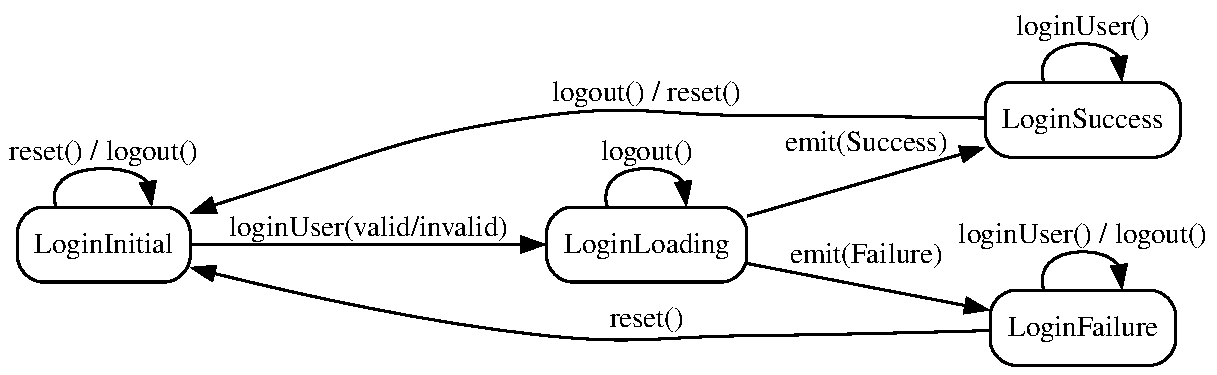
\includegraphics[width=0.8\textwidth]{dot/login.pdf}
\caption{Пример графа автомата состояний для гипотетического LoginCubit.}
\label{fig:cubit_fsm_example}
\end{figure}

\vspace{2cm}

\begin{figure}[!htb]
\centering
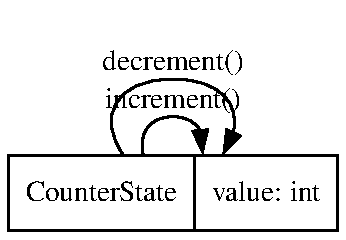
\includegraphics[width=0.7\textwidth]{dot/counter.pdf}
\caption{Пример графа автомата состояний для простого CounterCubit.}
\label{fig:cubit_fsm_example_2}
\end{figure}

\end{document}